\newpage
\appendix
\pagenumbering{roman}
\chapter{Experimenty so syntetickým gradientom}
\label{SGexperimets}
% pravdepodobne nepravdivá informácia

V kapitole \ref{BPlambdaAlgoritmus} sme uviedli algoritmus $BP(\lambda)$ ktorý umožňuje neurónovej sieti trénovanie kombináciou dvoch gradientov. Ide o gradient šírený z vyššej vrstvy a syntetický gradient poskytnutý modulom syntetického gradientu. Výber z týchto dvoch gradientov je podmienený parametrom $\lambda$. 

\iffalse
Pri klasifikácii sa v etape trénovania neurónovej siete použila modifikácia algoritmu $BP(\lambda)$. Každá vrstva neurónovej siete na úpravu váh použila spätne šírený gradient vždy s pravdepodobnosťou $p_{update}$. Komunikačnú medzeru vypĺňa DNI ktoré poskytuje syntetický gradient. Syntetický gradient je použitý vždy s pravdepodobnosťou $1-p_{update}$.


V tomto experimente bolo dokopy vykonaných 100 rôznych trénovaní, pri ktorých bola zvolená vždy iná hodnota $p_{update}$ z rozsahu $\langle 0, 1\rangle$. Výsledky tohto experimentu je možné vidieť na obrázku \ref{vysledkyExperimentuBpLambda} a to \textbf{s} a \textbf{bez} použitia dodatočnej informácie $c$. Ako si môžeme všimnúť, pri využití spätne šíreného gradientu s pravdepodobnosťou $p\textsubscript{update}=0.2$ je neurónová sieť stále schopná klasifikovať vstupné dáta s chybou len 2\%. Prekvapivo, v prípade syntetického gradientu generovaného s využitím informácie o skutočnej hodnote $c$ sa pri vyššej hodnote $p\textsubscript{update}$ znižuje presnosť neurónovej siete \cite{Jaderberg2016}.
\fi

Zdroj \cite{Jaderberg2016} uviedol experiment, v ktorom použil konvolučnú neurónovú sieť na spracovanie dátovej sady MNIST. Jedná sa o dátovu sadu obsahujúcu rukou-písané čísla od 0 do 9 \cite{yann1998mnist}. Cieľom konvolučnej neurónovej siete bola klasifikácia jednotlivých rukou-písaných číslic na numerické hodnoty 0-9. V etape trénovania bola použitá metóda ktorá kombinuje využitie syntetického gradientu a spätne šíreného gradientu. Pri tomto experimente si každá vrstva upravila svoje váhy vždy za pomoci syntetického gradientu obdržaného od DNI. Po úplnom dokončení fázy dopredného šírenia sa vykonala fáza spätného šírenia chyby vždy s pravdepodobnosťou $p_{update}$. Vo fáze spätného šírenia chyby boli upravované váhy jednotlivých vrstiev a aj váhy modulov syntetického gradientu. DNI vypĺňa komunikačnú medzeru spätného šírenia chyby a zabezpečuje úpravu váh v každej iterácii trénovania \cite{Jaderberg2016}.

Experiment tiež pozoroval, aký vplyv na neurónovú sieť má dodatočná informácia $c$ pre modul syntetického gradientu. Ako dodatočná informácia bola poskytnutá supervízia, skutočná hodnota rukou-písanej číslice.

V tomto experimente bolo dokopy vykonaných 100 trénovaní, pri ktorých bola zvolená vždy iná hodnota $p\textsubscript{update}$ z rozsahu $\langle 0, 1\rangle$. Výsledky experimentu je možné vidieť z grafov na Obrázku \ref{vysledkyExperimentuBpLambda}. 

Neurónová sieť je schopná klasifikovať jednotlivé dátove vzorky s chybou 2\% už v prípade pravdepodobnosti aktivácie spätného šírenia chyby $p_{update}=0,2$ \cite{Jaderberg2016}. Využitím dodatočnej informácie $c$ pre moduly syntetického gradientu sa zvyšovaním pravdepodobnosti $p_{update}$ znižuje presnosť neurónovej siete.


\begin{figure}
%vlozenie samotneho obrazku vycentrovaneho a vhodnej velkosti
%obrazok je v subore images/cervik.png
\centerline{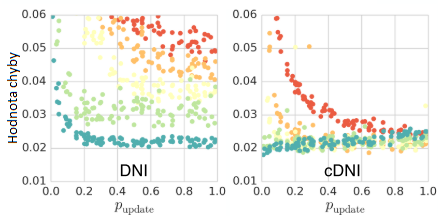
\includegraphics[width=0.6\textwidth]{images/vysledkyExperimentuBpLambda}}
%popis obrazku
\caption[Podmienenie aktivácie spätného šírenia chyby pravdepodobnosťou $p\textsubscript{update}$]{Grafy znázorňujú vývoj chyby konvolučnej neurónovej siete trénovanej na klasifikáciu dátovej sady MNIST \cite{yann1998mnist}. Neurónová sieť upravuje váhy skrytých vrstiev využitím syntetického gradientu. Po dokončení fázy dopredného šírenia sa vykoná fáza spätného šírenia chyby s pravdepodobnosťou $p_{update}$. Graf vľavo znázorňuje, aký vplyv má pravdepodobnosť aktivácie fázy spätného šírenia $p_{update}$ na chybu neurónovej siete využívajúcu syntetický gradient (DNI). Graf vpravo zobrazuje, aký vplyv má pravdepodobnosť aktivácie fázy spätného šírenia chyby $p_{update}$ na neurónovú sieť využívajúcu syntetický gradient generovaný modulom syntetického gradientu s dodatočná informácia o supervízii $c$ (cDNI) \cite{Jaderberg2016}.}
%id obrazku, pomocou ktoreho sa budeme na obrazok odvolavat
\label{vysledkyExperimentuBpLambda}
\end{figure}

\section{Rozšírenie modulu syntetického gradientu}
\label{experiment_SG2}

Na začiatku kapitoly sme opísali experiment z \cite{Jaderberg2016}, pri ktorom bola konvolučná neurónová sieť aplikovaná na klasifikáciu dátovej sady MNIST \cite{yann1998mnist}. Táto neurónová sieť vykonávala na každej skrytej vrstve lineárnu klasifikáciu realizovanú dávkovou normalizáciou \cite{Ioffe2015} a transformáciu dát pomocou ReLU (z angl. Rectified Linear Unit) \cite{Xu2015}. 

V ďalšom experimente \cite{Jaderberg2016} bola použitá podobná konvolučná neurónová sieť ktorá obsahuje tri skryté vrstvy a jednu klasifikačnú, výstupnú vrstvu. Ku každej skrytej vrstve je pripojený samostatný modul syntetického gradientu. Experiment pozoroval vplyv syntetického gradientu a hĺbky neurónovej siete na klasifikáciu rukou-písaných čísel dátovej sady MNIST a rozpoznávanie objektov dátovej sady CIFAR-10 \cite{Krizhevsky09learningmultiple}. V každom pozorovaní je hĺbka neurónovej siete menená medzi 3 až 6 skrytými vrstvami. 

Výsledok experimentu je možné vidieť v tabuľke \ref{compareDNIandCDNI}. Využitie DNI v praxi skutočne funguje \cite{Jaderberg2016}. DNI za cenu drobného poklesu presnosti predikcie, umožňuje úplne odstrániť \textit{uzamknutie úpravy váh} a \textit{uzamknutie v smere spätného šírenia chyby}. 

Experiment tiež pozoroval vplyv dodatočnej informácie o supervízii $c$ poskytnutej modulom syntetického gradientu, na presnosť predikcie neurónovej siete. Z tabuľky \ref{compareDNIandCDNI} je možné vidieť, že poskytnutím dodatočnej informácie $c$ je možné trénovať neurónovú sieť s ešte menšou degradáciou presnosti ako v prípade využitia štandardného syntetického gradientu \cite{Jaderberg2016}. Toto tvrdenie vyplýva z porovnania presnosti predikcie na dátovej sade CIFAR-10. Zatiaľ čo neurónová sieť pozostávajúca z piatich skrytých vrstiev, využívajúca štandardný syntetický gradient má chybu 46.9\%, tak tá istá neurónová sieť, využívajúca syntetický gradient generovaný s využitím dodatočnej informácie $c$ má chybu predikcie 43.5\%. 

Zdroj \cite{Jaderberg2016} nakoniec uviedol, že vykonal experiment pri ktorom trénoval neurónovú sieť ktorá mala viac ako 21 skrytých vrstiev. Táto neurónová sieť využívala výhradne syntetický gradient generovaný modulom syntetického gradientu s dostupnou dodatočnou informáciou $c$ a hodnota chyby bola 2\%.

\begin{table}
% v tabulke sa popis zvykne davat nad tabulku
\caption[Porovnanie chyby neurónovej siete trénovanej rôznymi typmi gradientu]{Tabuľka zobrazuje chybu predikcie konvulenčnej neurónovej siete trénovanej na rozpoznávanie obrazu z dátových sád MNIST a CIFAR-10. Prvý stĺpec udáva informáciu o hĺbke neurónovej siete, kde daná hodnota predstavuje počet skrytých vrstiev. Pre každú dátovú sadu bola použitá tá istá neurónová sieť. Tabuľka obsahuje hodnoty chyby neurónovej siete využívajúcej gradient šírený spätnou propagáciou chyby (Bprop), syntetický gradient (DNI) alebo syntetický gradient obohátený o dodatočnú informáciu $c$ (cDNI) \cite{Jaderberg2016}.}
%id tabulky
\label{compareDNIandCDNI}
% tu zacina samotna tabulka
\begin{center}
\begin{tabular}{cc|ccc|ccc}
\toprule
      &       & \multicolumn{3}{c|}{MNIST (\% Chyba)} & \multicolumn{3}{c}{CIFAR-10 (\% Chyba)} \\
\midrule
\multicolumn{2}{c|}{Počet vrstiev} & Bprop & DNI  & cDNI  & Bprop & DNI & cDNI \\ \hline
\hline
\multicolumn{2}{c|}{3} & 2,0 & 1,9 & 2,2 & 43,5 & 42,5 & 48,5 \\
\multicolumn{2}{c|}{4} & 1,8 & 2,2 & 1,9 & 43,0 & 45,0 & 45,1 \\
\multicolumn{2}{c|}{5} & 1,8 & 3,4 & 1,7 & 41,7 & 46,9 & 43,5 \\
\multicolumn{2}{c|}{6} & 1,8 & 4,3 & 1,6 & 42,0 & 49,7 & 46,8 \\
\hline
%(many lines omitted)
\bottomrule
\end{tabular}%
\end{center}
\end{table}

Na tento experiment sme sa zamerali predovšetkým preto, aby sme zistili aký vplyv má syntetický gradient na neurónovú sieť, ktorá vykonáva lineárnu klasifikáciu realizovanú dávkovou normalizáciou a ReLU. Skutočnosť, že implementácia syntetického gradientu na takýto typ neurónovej siete nemá signifikantne negativný vplyv na presnosť neurónovej siete je pre nás pozitívna. Pozitívna vzhľadom k tomu, že ďalšia časť práce sa bude venovanáť reziduálnym sieťam ktoré využívajú dávkovú normalizáciu a ReLU. V tomto ohľade je pre nás nevyhnutné disponovať informáciou o tom, aký efekt syntetického gradientu na takúto sieť máme očakávať.

\chapter{Experimenty modifikácie reziduálneho bloku}

\section{Vplyv architektúry reziduálneho bloku na reziduálnu sieť}

\begin{table}[h]
% v tabulke sa popis zvykne davat nad tabulku
\caption[Porovnanie architektúr reziduálneho bloku]{Pozorovanie vplyvu architektúry reziduálneho bloku na chybu predikcie reziduálnej siete. Pozorovanie bolo vykonané na dvoch reziduálnych sieťach. Reziduálna sieť so 110 skrytými konvolučnými vrstvami (ResNet-110) a reziduálna sieť so 164 skrytými konvolučnými vrstvami (ResNet-164). Obidve neurónové siete boli trénované na rozpoznávanie obrazu z dátovej sady CIFAR-10 \cite{He2016}. Vizualizáciu pozorovaných architektúr reziduálnych blokov je možné vidieť na Obrázku \ref{fig:architectures_of_residual_blocks}}
%id tabulky
\label{compareArchitectures}
% tu zacina samotna tabulka
\begin{center}
\begin{tabular}{l|c|c|c}
\toprule
\multicolumn{2}{c}{} & \multicolumn{2}{c}{chyba (\%)} \\
\midrule
Architektúra & Obrázok & ResNet-110  & ResNet-164\\ \hline
\hline
pôvodný reziduálny blok          & Obr. \ref{fig:architectures_of_residual_blocks} a) & 6,61 & 5,93 \\
dávková normalizácia po sčítaním & Obr. \ref{fig:architectures_of_residual_blocks} b) & 8,17 & 6,50 \\
ReLu pred sčítaním               & Obr. \ref{fig:architectures_of_residual_blocks} c) & 7,84 & 6,14 \\
ReLu predaktivácia               & Obr. \ref{fig:architectures_of_residual_blocks} d) & 6,71 & 5,91 \\
\textbf{úplná predaktivácia}     & Obr. \ref{fig:architectures_of_residual_blocks} e) & \textbf{6,37} & \textbf{5,46} \\
\hline
%(many lines omitted)
\bottomrule
\end{tabular}%
\end{center}
\end{table}
\newpage

\section{Vplyv architektúry identitného prepojenia na reziduálnu sieť}

\begin{table}[h]
% v tabulke sa popis zvykne davat nad tabulku
\caption[Porovnanie rôznych architektúr identitného prepojenia]{Porovnanie vplyvu transformácie identického zobrazenia prechodom identitným prepojením na presnosť reziduálnej siete. Pozorovaná reziduálna sieť bola trénovaná na rozpoznávanie obrazu z dátovej sady CIFAR-10. Pozostávala zo 110 skrytých konvolučných vrstiev (ResNet-110) obsahujúcich $3\times 3$ konvolučné filtre. Niektoré merania boli vykonané viackrát, s rôznymi počiatočnými hodnotami preferencií $b_g$ (z angl. bias). Slovo \textit{zlyhanie} je použité, ak hodnota chyby presiahla 20\% \cite{He2016}. Vizualizácia pozorovaných architektúr identitného prepojenia je možné vidieť na Obrázku \ref{fig:achitectures_of_identity_shortcut}.}
%id tabulky
\label{compareIdentityTransformations}
% tu zacina samotna tabulka
\begin{comment}
\begin{center}
\begin{tabular}{l|c|c|c|c|l}
\toprule
Architektúra    & Obrázok  & na prepojení   &  na $\mathcal{F}$    & chyba (\%) & poznámka \\ 
\hline
\hline
pôvodný & Fig \ref{fig:achitectures_of_identity_shortcut}(a) & 1 & 1 & \textbf{6,61} & \\
\hline
\multirow{3}{*}{constant scaling}   & \multirow{3}{*}{Fig \ref{fig:achitectures_of_identity_shortcut}(b)} & 0 & 1 & zlyhanie & \\
& & 0,5 & 1 & zlyhanie & \\
& & 0,5 & 0,5 & 12,35 &  \\
\hline
\multirow{3}{*}{exclusive gating}   & \multirow{3}{*}{Fig \ref{fig:achitectures_of_identity_shortcut}(c)} & $1-g(x)$ & $g(x)$ & zlyhanie & $b_g = 0$ to $5$\\
& & $1-g(x)$ & $g(x)$ & 8,70 & $b_g = -6$\\
& & $1-g(x)$ & $g(x)$ & 9,81 & $b_g = -7$\\
\hline
\multirow{2}{*}{shortcut-only gating}   & \multirow{2}{*}{Fig \ref{fig:achitectures_of_identity_shortcut}(d)} & $1-g(x)$ & 1 & 12,86 & $b_g = 0$\\
& & $1-g(x)$ & 1 & 6,91 & $b_g = -6$\\
\hline
$1\times1$ conv shortcut& Fig \ref{fig:achitectures_of_identity_shortcut}(e) & $1\times1$ conv & 1 & 12,22 \\
\hline
dropout shortcut & Fig \ref{fig:achitectures_of_identity_shortcut}(f) & dropout 0,5 & 1 & zlyhanie \\
\hline
%(many lines omitted)
\bottomrule
\end{tabular}%
\end{center}
\end{comment}

\begin{center}
\begin{tabular}{l|c|c|l}
\toprule
Architektúra    & Obrázok  & chyba (\%) & poznámka \\ 
\hline
\hline
pôvodné identitné prepojenie & Obr. \ref{fig:achitectures_of_identity_shortcut} a) & \textbf{6,61} & \\
\hline
konštantné škálovanie   & Obr. \ref{fig:achitectures_of_identity_shortcut} b) & 12,35 &  \\
\hline
\multirow{3}{*}{exkluzívne hradlovanie}  & \multirow{3}{*}{Obr. \ref{fig:achitectures_of_identity_shortcut} c)} & zlyhanie & $b_g = 0$ to $5$\\
& & 8,70 & $b_g = -6$\\
& & 9,81 & $b_g = -7$\\
\hline
\multirow{2}{*}{hradlovanie v rámci prepojenia}   & \multirow{2}{*}{Obr. \ref{fig:achitectures_of_identity_shortcut} d)} & 12,86 & $b_g = 0$\\
& & 6,91 & $b_g = -6$\\
\hline
$1\times1$ konvulenčné prepojenie & Obr. \ref{fig:achitectures_of_identity_shortcut} e) & 12,22 \\
\hline
stochastické vynechávanie prepojenia (dropout)& Obr. \ref{fig:achitectures_of_identity_shortcut} f) & zlyhanie & \\
\hline
%(many lines omitted)
\bottomrule
\end{tabular}%
\end{center}

\end{table}

\chapter{Technická dokumentácia}

\section{Trénovania odšumujúceho autoenkódera}
\label{train_DAE}

Funkcia trénovania odšumujúceho autoenkódera (DAE) \mintinline{Python}{trainDAE()} je obsiahnutá v súbore \mintinline{Python}{denoisingAutoEncoder.py}. Funkcia ako parametre prijíma referenčnú vzorku, cestu k jednotlivým vzorkám dátovej sady, identifikátor referenčnej vzorky, zoznam vzoriek ktoré je možné použiť na trénovanie, identifikátory relevantných markerov, formát súboru v ktorom sú vzorky uložené, miera zašumenia vzoriek pri trénovaní DAE, identifikátor potreby odšumenia dát, identifikátor potreby trénovania nového DAE a cesta, kde bude nový DAE uložený. 

V prvej fáze trénovania DAE sú načítané všetky vzorky dátovej sady (okrem referenčnej vzorky) do pamäte a následne sú vyselektované tie záznamy, ktoré neobsahujú prázdne hodnoty. Načítané vzorky sú normalizované logaritmickou tranformáciou definovanou ako opisuje výraz \ref{log_transf}. Normalizované vzorky z dátovej sady sú následne spojené s referenčnou vzorkou za účelom rozšírenia rozmanitosť dátovej sady.  Následne je z novovytvorenej dátovej sady (združujúcej referenčnú vzorku a všetky vzorky z dátovej sady) vytvorená kópia ktorá je zašumená mierou zašumenia definovanou pri volaní funkcie \mintinline{Python}{trainDAE()}. Zašumená dátová sada predstavuje trénovaciu sadu určenú na trénovanie DAE, zatiaľ čo pôvodná dátová sada je použitá pri vypočítavaní hodnoty chyby predikcie ako cieľová vzorka (supervízia).

Ak je nie je potrebné trénovať nový DAE, tak autoenóder je načítaný z disku. V opačnom prípade je DAE zostrojený pomocou jednej vstupnej vrstvy (inštancia triedy \mintinline{Python}{Input}, obsiahnutej v knižnici \mintinline{Python}{Keras}) a troch plne-prepojených váhových vrstiev (inštancia triedy \mintinline{Python}{Dense}, obsiahnutej v knižnici \mintinline{Python}{Keras}). Všetky skryté vrstvy disponujú $l_2$ regularizáciou váh, kde hodnota $l_2$ regularizácie je $10^{-2}$. Prvé dve vrstvy DAE využívajú aktivačnú funkciu ReLU, pričom výstupná vrstva DAE využíva lineárnu aktivačnú funkciu.

Jednotlivé vrstvy DAE sú zapuzdrené v objekte triedy \mintinline{Python}{Model}, obsiahnutej v knižnici \mintinline{Python}{Keras}. Zostrojenie DAE je realizované metódou \mintinline{Python}{compile()} triedy \mintinline{Python}{Model}. Metóda \mintinline{Python}{compile()} prijíma ako parametre metódu úpravy váh (v našom prípade RMSPropOptimalizer \cite{Goh1995}) a typ chybovej funkcie (v našom prípade funkcia priemernej kvadratickej chyby (MSE, z angl. Mean Squared Error)). Aktivácia trénovania je realizovaná metódou \mintinline{Python}{fit()} triedy \mintinline{Python}{Model}. Trénovanie DAE pozostáva z 80 iterácii a veľkosťou dávky 128. Natrénovaný DAE je následne uložený na disk.

Výstupom funkcie \mintinline{Python}{trainDAE()} je natrénovaný DAE, ktorý je možné použiť na odšumenie vstupných dát.

\section{Odšumenie vstupných dát pomocou ošumujúceho autoenkódera}
\label{predict_DAE}

Odšumenie vstupných dát pomocou DAE je realizované funkciou \mintinline{Python}{predictDAE()}, ktorá prijíma ako parametre dáta ktoré budú odšumené, natrénovaný autoenkóder použitý na odšumenie vstupných dát a identifikátor potreby odšumenia dát. Ako sme uviedli v Prílohe \ref{train_DAE}, natrénovaný autoenkóder je objektom triedy \mintinline{Python}{Model}, obsiahnutej v knižnici \mintinline{Python}{Keras}. Odšumenie dát je vykonané volaním metódy \mintinline{Python}{predict()} triedy \mintinline{Python}{Model}, ktorá prijíma ako parameter vstupnú vzorku, ktorá má byť daným autoenkóderom odšumená. 

Výstupom funkcie \mintinline{Python}{predictDAE()} je inštancia triedy \mintinline{Python}{Sample}, obsiahnutej v súbore \mintinline{Python}{denoisingAutoEncoder.py}, ktorej atribútmi sú:
\begin{enumerate}
    \item \mintinline{Python}{X} - odšumené vstupné dáta
    \item \mintinline{Python}{y} - pôvodné identifikátory tried jednotlivých buniek
\end{enumerate}

\section{Trénovanie bunkového klasifikátora}
\label{trainFF}

Trénovanie bunkového klasifikátora je realizované volaním funkcie \mintinline{Python}{trainClassifier()}, obsiahnutej v súbore \mintinline{Python}{feedforwardClassifier.py}. Funkcia ako parametre prijíma trénovaciu vzorku (v našom prípade referenčná vzorka), formát súboru v ktorom sú uložené vzorky dátovej sady, identifikátor referenčnej vzorky v dátovej sade, zoznam veľkostí skrytých vrstiev klasifikátora, typ aktivačnej funkcie skrytých vrstiev klasifikátora, hodnotu $l_2$ regularizácie váh skrytých jednotlivých vrstiev klasifikátora a cestu, kde bude novonatrénovaný klasifikátor uložený.

V úvode trénovania sú z trénovacej vzorky odstránené všekty záznamy (bunky), ktoré prislúchajú triede $0$ (trida neurčitých/neznámych buniek). Odstránenie neurčitých buniek umožňuje trénovať klasifikátor len na bunkách, ktorých trieda je známa a klasifikátor je tak schopný lepšie predikovať známe triedy jednotlivých buniek. 

Bunkový klasifikátor je zostrojený z jednej vstupnej vrstvy (objekt triedy \mintinline{Python}{Input}, obsiahnutý v knižnici \mintinline{Python}{Keras}) a troch skrytých plneprepojených váhových vrstvách (objekt triedy \mintinline{Python}{Dense}, obsiahnutý v knižnici \mintinline{Python}{Keras}). Veľkosť vstupnej vrstvy je rovná počtu parametrov trénovacej vzorky (v našom prípade počet markerov v referenčnej vzorke). Veľkosti skrytých vrstiev sú inicializované na základe zoznamu veľkostí skrytých vrstiev poskytnutého pri volaní funkcie \mintinline{Python}{trainClassifier()}. Jednotlivé skryté vrstvy vykonávajú $l_2$ regularizáciu váh s hodnotou $l_2$ regularizácie uvedenej v parametroch volania funkcie \mintinline{Python}{trainCLassifier()}. Aktivačná funkcia skrytých vrstiev je definovaná v parametroch pri volaní funkcie \mintinline{Python}{trainClassifier()}.

Po deklarovaní skrytých vrstiev nasleduje deklarácia výstupnej vrstvy. Výstupná vrstva je objektom triedy \mintinline{Python}{Dense}, obsiahnutej v knižnici \mintinline{Python}{Keras} a jej veľkosť je rovná počtu tried, vyskytujúcich sa v trénovecej vzorke. Aktivačná funkcia výstupnej vrstvy je funkcia \textit{Softmax} \cite{Goh1995}.

Deklarované vrstvy klasifikátora (počnúc vstupnou vrstvou a končiac výstupnou vrstvou) sú zapuzdrené v objekte triedy \mintinline{Python}{Model}, obsiahnutej v knižnici \mintinline{Python}{Keras}. Zostrojenie modelu klasifikátora je realizované metódou \mintinline{Python}{compile()}, obsiahnutou v triede \mintinline{Python}{Model}. Funkcia \mintinline{Python}{compile()} prijíma ako parametre metódu úpravy váh (v našom prípade RMSPropOptimizer \cite{Goh1995}) a typ chybovej funkcie (v našom prípade funkcia riedkej kategorickej krížovej entropie (SCCE, z angl. Sparse Categorical CrossEntropy)).

Zostrojený model je následne trénovaný metódou \mintinline{Python}{fit()}, obsiahnutou v triede \mintinline{Python}{Model}. Trénovanie bunkového klasifikátore je realizované 80 iteráciami s veľkosťou trénovacej dávky 128. Trénovanie klasifikátora využíva dynamický krok učenia definovaný ako opisuje \ref{dyna_lr}. Pretrénovanie klasifikátora je ošetrené implementáciou funkcie predčasného zastavenia \mintinline{Python}{EarlyStopping()}, obsiahnutej v knižnici \mintinline{Python}{Keras}.

Natrénovaný klasifikátor je uložený na disk. Výstupom funkcie \mintinline{Python}{trainClassifier()} je natrénovaný klasifikátor, resp. objekt triedy \mintinline{Python}{Model}.

\section{Gatovanie pomocou bunkového klasifikátora}
\label{gateFF}

Gatovanie, resp. klasifikovanie jednotlivých buniek vzsupnej vzorky do diskrétnych skupín je realizované funkciou \mintinline{Python}{prediction()}, obsiahnutou v súbore \mintinline{Python}{feedforwardClassifier.py}. Funkcia \mintinline{Python}{prediction()} prijíma ako parametre vzorku dát, ktoré budú klasifikované (gatované), formát súboru vzoriek dátovej sady, identifikátor referenčnej vzorky a natrénovaný klasifikátor, ktorý bude použitý na klasifikovanie vstupnej vzorky.

Ako je uvedené v Prílohe \ref{trainFF}, klasifikátor je inštanciou triedy \mintinline{Python}{Model}, obsiahnutej v knižnici \mintinline{Python}{Keras}. Klasifikovanie vzorky je realizované volaním metódy \mintinline{Python}{predict()} nad daným objektom klasifikátora. Metóda \mintinline{Python}{predict()} ako parametre prijíma vzorku dát, ktoré majú byť predikované. Výstupom metódy \mintinline{Python}{predict()} je hodnota pravdepodobností priradenia každej buniek do jednotlivých tried (napr. [0.27, 0.18, 0.04. 0.79]). V ďalšom kroku je vybraný index tej hodnoty pravdepodobnosti, ktorá je pre každú bunku najvyššia (vo vyššie uvedenom prípade ide o index 3). Všetky vybrané indexy sú následne inkrementované o 1 aby bol dodržaný pôvodný konsenzus identifikátorov bunkových tried (trieda ktorá má identifikátor 1 sa nachádza na indexe 0 a preto je potrebné inkrementovať všetky indexy o hodnotu 1). Následne všetky bunky, ktorých najvyššia pravdepodobnosť priradenia do nejakej skupiny je nižšia ako hodnota 0.4, sú priradené do skupiny s identifikátorom 0 (skupina neurčitých/neznámych buniek).

Výstupom funkcie \mintinline{Python}{prediction()} je hodnota presnosti gatovania, $F1$ skôre dosiahnuté pri gatovaní daným kalsifikátorom a klasifikované triedy buniek vstupnej vzorky.

\chapter{Používateľská príručka}

Táto kapitola opisuje sekvenciu krokov, ktoré je potrebné vykonať za účelom korektného spustenia programu. Používateľská príručka sa orientuje na spusteniu programu na platforme \textit{Mac OS}.

Prvý krok predstavuje nainštalovanie spúšťacej jednoty programovacieho jazyka \textit{Python 3}. Na nainštalovanie spúšťacej jednotky je najprv potrebné nainštalovať správcu balíkov pre systém \textit{Mac OS}, \textit{Homebrew}. Inštalácia správcu balíkov \textit{Homebrew} je realizovaná nasledujúcim príkazom:

\begin{Verbatim}[breaklines=true, breakanywhere=true]
ruby -e "\$(curl -fsSLhttps://raw.githubusercontent.com/Homebrew/install/master/install)"
\end{Verbatim}

Pomocou správcu balíkov \textit{Homebrew} je možné nainštalovať spúšťaciu jednotku programovacieho jazyka \textit{Python 3}, ako

\begin{Verbatim}[breaklines=true, breakanywhere=true]
brew install python
\end{Verbatim}

Správca balíkov \textit{Homebrew} pri inštalácii spúšťacej jednotky programovacieho jazyka \textit{Python} nainštaluje aj správcu balíkov jazyka \textit{Python}, \mintinline{Python}{pip}. Správca balíkov \mintinline{Python}{pip} umožňuje sťahovať všetky potrebné knižnice a rozšírenia programovacieho jazyka \textit{Python}. Nasledujúci zoznam opisuje všetky knižnice ktoré je potrebné nainštalovať pred spustením programu a príkazy, ktorými je možné dané knižnice nainštalovať.

\textbf{Keras}
\begin{Verbatim}[breaklines=true, breakanywhere=true]
pip install keras
\end{Verbatim}

\textbf{Numpy}
\begin{Verbatim}[breaklines=true, breakanywhere=true]
pip install numpy
\end{Verbatim}

\textbf{Pandas}
\begin{Verbatim}[breaklines=true, breakanywhere=true]
pip install pandas
\end{Verbatim}

\textbf{Scikit Learn}
\begin{Verbatim}[breaklines=true, breakanywhere=true]
pip install -U scikit-learn
\end{Verbatim}

\textbf{FCS parser}
\begin{Verbatim}[breaklines=true, breakanywhere=true]
pip install fcsparser
\end{Verbatim}

\textbf{Random}
\begin{Verbatim}[breaklines=true, breakanywhere=true]
pip install random2
\end{Verbatim}

\textbf{Mathplotlib}
\begin{Verbatim}[breaklines=true, breakanywhere=true]
pip install -U matplotlib
\end{Verbatim}

\textbf{Tqdm}
\begin{Verbatim}[breaklines=true, breakanywhere=true]
pip install tqdm
\end{Verbatim}

\textbf{TensorFlow}
\begin{Verbatim}[breaklines=true, breakanywhere=true]
pip install tensorflow
\end{Verbatim}

Po nainštalovaní všetkých knižníc je možné prejsť k samotnému spusteniu programu. Z priloženého kompaktného disku skopírujeme do počítača adresár \mintinline{Python}{BP_Hanincik}. V konzole sa pomocou príkazu \mintinline{Python}{cd} presunieme do novovytvorenej kópie adresára \mintinline{Python}{BP_Hanincik}. Následne sa presunieme do podadresára \mintinline{Python}{src} (znovu používame príkaz \mintinline{Python}{cd}). V adresári \mintinline{Python}{src} sa nachádza spustiteľný program \mintinline{Python}{DeepCyTOF.py}, napísaný v programovacom jazyku \mintinline{Python}{Python}. Program \mintinline{Python}{DeepCyTOF.py} spustíme príkazom 

\begin{Verbatim}[breaklines=true, breakanywhere=true]
python DeepCyTOF.py
\end{Verbatim}

Pri spustení je potrebné skontrolovať používateľské práva k súboru \mintinline{Python}{DeepCyTOF.py}. Výsledok programu je možné nájsť v adresári \mintinline{Python}{results}, ktorý obsahuje:

\begin{itemize}
    \item zdrojové vzorky kalibrované pomocou MMD-ResNet využívajúcej algoritmus syntetického gradientu (vo formáte \mintinline{Python}{csv})
    \item predikované triedy jednotlivých buniek zdrojových vzoriek (vo formáte \mintinline{Python}{csv})
    \item vizualizácia priebehu vývoja hodnoty MMD v čase trénovania MMD-ResNet (vo formáte \mintinline{Python}{png})
    \item vizualizácia priebehu vývoja hodnoty MMD v jednotlivých iteráciach trénovania MMD-ResNet (vo formáte \mintinline{Python}{png})
    \item vizualizácia vývoja \textit{F1 skóre} v priebehu trénovania MMD-ResNet (vo formáte \mintinline{Python}{png})
\end{itemize}

Každý z vytvorených súborov sa nachádza v samostatnom adresári s názvom korešpondujúcim názvu prislúchajúcej vzorky.

\chapter{Plán práce na riešení projektu}
\begin{enumerate}
    \item Implementácia a analýza metódy DeepCyTOF (December)
    \item Implementácia syntetického gradientu v reziduálnej sieti MMD-ResNet (Január-Február)
    \item Experimentovanie a pozorovanie vplyvu syntetického gradientu na presnosť predikcií metódy DeepCyTOF (Marec)
    \item Vyhodnocovanie experimentov (Apríl)
\end{enumerate}

Plnenie stanoveného plánu práce bolo vo veľkej miere dodržané. Veľké zadosťučinenie pri plnení plánu práce mala aj účasť na študentskej výskumnej konferencii \textit{IIT.SRC 2019}. Vzhľadom na skoré termíny odovzdania vedeckých príspevkov na danú konferenciu, bolo potrebné urýchliť prvú a druhú fázu implementácie (implementáciu a analýzu metódy DeepCyTOF a implementáciu syntetického gradientu v reziduálnej sieti MMD-ResNet). Prvotné výsledky implementácie boli nadobudnuté už pri prvom odovzdaní predbežnej verzie príspevku na študentskú konferenciu \textit{IIT.SRC 2019} (24.2.2019). 

Následne sme postupovali podľa plánu a všetok čas sme investovali do zlepšovania implementácie a ladenia hyperparametrov. Časový sklz nastal pri rozširovaní metódy DeepCyTOF o dodatočnú funkcionalitu umožňujúcu klasifikovať dátovú sadu poskytnutú Slovenskou Akadémiou Vied.

Okrem študentskej konferencie \textit{IIT.SRC 2019} sme našu prácu prezentovali ešte trikrát a to na rôznych seminároch. Výsledná práca zahŕňa splnenie všetkých stanovených požiadaviek v požadovanom rozsahu.